\documentclass[a4paper,twoside]{article}
% My LaTeX preamble file - by Nathaniel Dene Hoffman
% Credit for much of this goes to Olivier Pieters (https://olivierpieters.be/tags/latex)
% and Gilles Castel (https://castel.dev)
% There are still some things to be done:
% 1. Update math commands using mathtools package (remove ddfrac command and just override)
% 2. Maybe abbreviate \imath somehow?
% 3. Possibly format for margin notes and set new margin sizes
% First, some encoding packages and useful formatting
%--------------------------------------------------------------------------------------------
\usepackage{import}
\usepackage{pdfpages}
\usepackage{transparent}
\usepackage[l2tabu,orthodox]{nag}   % force newer (and safer) LaTeX commands
\usepackage[utf8]{inputenc}         % set character set to support some UTF-8
                                    %   (unicode). Do NOT use this with
                                    %   XeTeX/LuaTeX!
\usepackage[T1]{fontenc}
\usepackage[english]{babel}         % multi-language support
\usepackage{sectsty}                % allow redefinition of section command formatting
\usepackage{tabularx}               % more table options
\usepackage{booktabs}
\usepackage{titling}                % allow redefinition of title formatting
\usepackage{imakeidx}               % create and index of words
\usepackage{xcolor}                 % more colour options
\usepackage{enumitem}               % more list formatting options
\usepackage{tocloft}                % redefine table of contents, new list like objects
\usepackage{subfiles}               % allow for multifile documents

% Next, let's deal with the whitespaces and margins
%--------------------------------------------------------------------------------------------
\usepackage[centering,margin=1in]{geometry}
\setlength{\parindent}{0cm}
\setlength{\parskip}{2ex plus 0.5ex minus 0.2ex} % whitespace between paragraphs

% Redefine \maketitle command with nicer formatting
%--------------------------------------------------------------------------------------------
\pretitle{
  \begin{flushright}         % align text to right
    \fontsize{40}{60}        % set font size and whitespace
    \usefont{OT1}{phv}{b}{n} % change the font to bold (b), normally shaped (n)
                             %   Helvetica (phv)
    \selectfont              % force LaTeX to search for metric in its mapping
                             %   corresponding to the above font size definition
}
\posttitle{
  \par                       % end paragraph
  \end{flushright}           % end right align
  \vskip 0.5em               % add vertical spacing of 0.5em
}
\preauthor{
  \begin{flushright}
    \large                   % font size
    \lineskip 0.5em          % inter line spacing
    \usefont{OT1}{phv}{m}{n}
}
\postauthor{
  \par
  \end{flushright}
}
\predate{
  \begin{flushright}
  \large
  \lineskip 0.5em
  \usefont{OT1}{phv}{m}{n}
}
\postdate{
  \par
  \end{flushright}
}

% Mathematics Packages
\usepackage[Gray,squaren,thinqspace,cdot]{SIunits}      % elegant units
\usepackage{amsmath}                                    % extensive math options
\usepackage{amsfonts}                                   % special math fonts
\usepackage{mathtools}                                  % useful formatting commands
\usepackage{amsthm}                                     % useful commands for building theorem environments
\usepackage{amssymb}                                    % lots of special math symbols
\usepackage{mathrsfs}                                   % fancy scripts letters
\usepackage{cancel}                                     % cancel lines in math
\usepackage{esint}                                      % fancy integral symbols
\usepackage{relsize}                                    % make math things bigger or smaller
%\usepackage{bm}                                         % bold math!
\usepackage{slashed}

\newcommand\ddfrac[2]{\frac{\displaystyle #1}{\displaystyle #2}}    % elegant fraction formatting
\allowdisplaybreaks[1]                                              % allow align environments to break on pages

% Ensure numbering is section-specific
%--------------------------------------------------------------------------------------------
\numberwithin{equation}{section}
\numberwithin{figure}{section}
\numberwithin{table}{section}

% Citations, references, and annotations
%--------------------------------------------------------------------------------------------
\usepackage[small,bf,hang]{caption}        % captions
\usepackage{subcaption}                    % adds subfigure & subcaption
\usepackage{sidecap}                       % adds side captions
\usepackage{hyperref}                      % add hyperlinks to references
\usepackage[noabbrev,nameinlink]{cleveref} % better references than default \ref
\usepackage{autonum}                       % only number referenced equations
\usepackage{url}                           % urls
\usepackage{cite}                          % well formed numeric citations
% format hyperlinks
\colorlet{linkcolour}{black}
\colorlet{urlcolour}{blue}
\hypersetup{colorlinks=true,
            linkcolor=linkcolour,
            citecolor=linkcolour,
            urlcolor=urlcolour}

% Plotting and Figures
%--------------------------------------------------------------------------------------------
\usepackage{tikz}          % advanced vector graphics
\usepackage{pgfplots}      % data plotting
\usepackage{pgfplotstable} % table plotting
\usepackage{placeins}      % display floats in correct sections
\usepackage{graphicx}      % include external graphics
\usepackage{longtable}     % process long tables

% use most recent version of pgfplots
\pgfplotsset{compat=newest}

% Misc.
%--------------------------------------------------------------------------------------------
\usepackage{todonotes}  % add to do notes
\usepackage{epstopdf}   % process eps-images
\usepackage{float}      % floats
\usepackage{stmaryrd}   % some more nice symbols
\usepackage{emptypage}  % suppress page numbers on empty pages
\usepackage{multicol}   % use this for creating pages with multiple columns
\usepackage{etoolbox}   % adds tags for environment endings
\usepackage{tcolorbox}  % pretty colored boxes!


% Custom Commands
%--------------------------------------------------------------------------------------------
\newcommand\hr{\noindent\rule[0.5ex]{\linewidth}{0.5pt}}                % horizontal line
\newcommand\N{\ensuremath{\mathbb{N}}}                                  % blackboard set characters
\newcommand\R{\ensuremath{\mathbb{R}}}
\newcommand\Z{\ensuremath{\mathbb{Z}}}
\newcommand\Q{\ensuremath{\mathbb{Q}}}
%\newcommand\C{\ensuremath{\mathbb{C}}}
\renewcommand{\arraystretch}{1.2}                                       % More space between table rows (could be 1.3)
\newcommand{\Cov}{\mathrm{Cov}}
\newcommand\D{\mathrm{D}}
\newcommand*{\dbar}{\ensuremath{\text{\dj}}}

\newcommand{\incfig}[2][1]{%
    \def\svgwidth{#1\columnwidth}
    \import{./figures/}{#2.pdf_tex}
}

% Custom Environments
%--------------------------------------------------------------------------------------------
\newcommand{\lecture}[3]{\hr\\{\centering{\large\textsc{Lecture #1: #3}}\\#2\\}\hr\markboth{Lecture #1: #3}{\rightmark}}   % command to title lectures
\usepackage{mdframed}
\theoremstyle{plain}
\newmdtheoremenv[nobreak]{theorem}{Theorem}[section]
\newtheorem{corollary}{Corollary}[theorem]
\newtheorem{lemma}[theorem]{Lemma}
\theoremstyle{definition}
\newtheorem*{ex}{Example}
\newmdtheoremenv[nobreak]{definition}{Definition}[section]
\theoremstyle{remark}
\newtheorem*{remark}{Remark}
\newtheorem*{claim}{Claim}
\AtEndEnvironment{ex}{\null\hfill$\diamond$}%
% Note: A proof environment is already provided in the amsthm package
\tcbuselibrary{breakable}
\newenvironment{note}[1]{\begin{tcolorbox}[
    arc=0mm,
    colback=white,
    colframe=white!60!black,
    title=#1,
    fonttitle=\sffamily,
    breakable
]}{\end{tcolorbox}}
\newenvironment{problem}{\begin{tcolorbox}[
    arc=0mm,
    breakable,
    colback=white,
    colframe=black
]}{\end{tcolorbox}}

% Header and Footer
%--------------------------------------------------------------------------------------------
% set header and footer
\usepackage{fancyhdr}                       % header and footer
\pagestyle{fancy}                           % use package
\fancyhf{}
\fancyhead[LE,RO]{\textsl{\rightmark}}      % E for even (left pages), O for odd (right pages)
\fancyfoot[LE,RO]{\thepage}
\fancyfoot[LO,RE]{\textsl{\leftmark}}
\setlength{\headheight}{15pt}


% Physics
%--------------------------------------------------------------------------------------------
\usepackage[arrowdel]{physics}      % all the usual useful physics commands
\usepackage{feyn}                   % for drawing Feynman diagrams
%\usepackage{bohr}                   % for drawing Bohr diagrams
%\usepackage{tikz-feynman}
\usepackage{elements}               % for quickly referencing information of various elements
\usepackage{tensor}                 % for writing tensors and chemical symbols

% Finishing touches
%--------------------------------------------------------------------------------------------
\author{Nathaniel D. Hoffman}

\title{33-765 Homework 3}
\date{\today}
\begin{document}
\maketitle

\section*{8. The Gamma Function}
One of the first ``special functions'' one learns about in college\textemdash after having covered exponentials, logarithms, and trigonometric functions in high school\textemdash is probably the Gamma function, $ \Gamma(x) $, which is usually defined as the following integral:
\begin{equation}
    \Gamma(x) = \int_{0}^{\infty} \dd{t} t^{x - 1} e^{-t} \quad x \in \C, \Re(x) > 0
\end{equation}
Prove the recurrence relation $ \Gamma(x+1) = x \Gamma(x) $ and deduce from it that $ \Gamma(N + 1) = N! $ for $ N \in \mathbb{N}_0 $. Also, calculate $ \Gamma\left( \frac{1}{2} \right) $.
\begin{problem}
    We prove the recurrence relation by integrating by parts ($ \int u \dd{v} = uv - \int v \dd{u} $), with
        \begin{align}
            \Gamma(x + 1) &= \int_{0}^{\infty} \dd{t} t^{x} e^{-t} \\
            &\begin{cases} u = t^{x} \\ \dd{u} = x t^{x-1} \\ \dd{v} = \dd{t} e^{-t} \\ v = - e^{-t}\end{cases} \\
            \Gamma(x + 1) &= \eval{-t^{x} \cancel{e^{-t}}}_{t=0}^{\infty} + \int_{0}^{\infty} x t^{x-1} e^{-t} \\
            &= x \Gamma(x)
        \end{align}
        Next, we want to show the relation between the Gamma function and the factorial.
        \begin{align}
            \Gamma(N + 1) &= N \Gamma(N) = N (N - 1) \Gamma(N - 1) = N (N - 1)(N - 2) \Gamma(N-2) = \cdots \\
            &= N (N - 1)(N - 2)\cdots(N-(N-1)) \Gamma(1)
        \end{align}
        where
        \begin{equation}
            \Gamma(1) = \int_{0}^{\infty} \dd{t} t e^{-t} = \eval{- \frac{t + 1}{e^{t}}}_{t=0}^{\infty} = 0 - (-1) = 1
        \end{equation}
        This is equivalent to the definition of the factorial:
        \begin{equation}
            N! = N(N-1)(N-2)\cdots\cancelto{1}{(N-(N-1))}
        \end{equation}
        Finally, we need to calculate $ \Gamma\left( \frac{1}{2} \right) $:
        \begin{equation}
            \Gamma\left( \frac{1}{2} \right) = \int_{0}^{\infty} \dd{t} \frac{1}{\sqrt{t}} e^{-t} 
        \end{equation}
        Next, make the substitution $ u^2 = t $, $ u = \sqrt{t} $, $ \dd{u} = \frac{\dd{t}}{2 \sqrt{t}} $:
        \begin{equation}
            \Gamma\left( \frac{1}{2} \right) = \int_{0}^{\infty} 2\dd{u} e^{- u^2}
        \end{equation}
        This function is even, so we can change the bounds of integration and divide by two:
        \begin{equation}
            \Gamma\left( \frac{1}{2} \right) = \int_{- \infty}^{\infty} e^{- u^2} \dd{u}
        \end{equation}
        This is now the form of an un-normalized Gaussian centered at $ \mu = 0 $ with a standard deviation of $ \sigma = \frac{1}{\sqrt{2}} $. If it was normalized, there would be an additional factor of $ \frac{1}{\sqrt{\pi}} $ multiplying it, and that would make the integral equal to $ 1 $:
        \begin{equation}
            \int_{- \infty}^{\infty} \frac{1}{\sqrt{\pi}} e^{- u^2} \dd{u} = 1
        \end{equation}
        so
        \begin{equation}
            \Gamma\left( \frac{1}{2} \right) = \sqrt{\pi}
        \end{equation}
\end{problem}

\section*{9. The Cauchy-Lorentz Distribution}
The p-density of the Cauchy-Lorentz distribution $ p_{x_0, a}(x) $ with location parameter $ x_0 $ and scale parameter $ a $ is defined as
\begin{equation}
    p_{x_0, a}(x) = \frac{a / \pi}{a^2 + (x - x_0)^2}.
\end{equation}
\begin{itemize}
    \item[1.] Show that $ p_{x_0, a}(x) $ is normalized. Also show that none of its higher moments exist.
        \begin{problem}
            To show that the distribution is normalized, we integrate over the domain and show that we get $ 1 $. I will assume it is okay if I know that the integral of $ \frac{1}{1 - x^2} = \arctan(x) $ is well known, so the $ a $ and $ x_0 $ just scale and shift the integral while the $ \frac{1}{\pi} $ factor can be brought outside:
            \begin{equation}
                \int_{- \infty}^{\infty} p_{x_0, a}(x) \dd{x} = \frac{1}{\pi} \eval{\arctan(\frac{x - x_0}{a})}_{- \infty}^{\infty} = \frac{1}{\pi} \left( \frac{\pi}{2} - \left( - \frac{\pi}{2} \right) \right) = 1
            \end{equation}
        To show that none of its higher moments exist, let's look at the first moment. For simplicity (and without loss of generality), I will take the location parameter to be $ x_0 = 0 $ and the scale parameter to be $ a = 1 $ (If the moments did exist, I could just reposition and scale them after this calculation):
        \begin{equation}
            \frac{1}{\pi} \int_{- \infty}^{\infty} \frac{x}{1 + x^2} \dd{x} = \frac{1}{2\pi} \eval{\ln(1 + x^2)}_{x= - \infty}^{\infty}
        \end{equation}
        The $ x^2 $ term in the logarithm makes this tricky. Both ends of the integral will evaluate to the same limit ($ \infty $) at the same speed (logarithmically), so if we take the integral as a limit:
        \begin{equation}
            \int_{- \infty}^{\infty} x p(x) \to \lim_{a \to \infty} \int_{-a}^{a} = \lim_{a \to \infty} \frac{1}{2 \pi} \ln(\frac{1+ a^2}{1 + a^2}) = \frac{1}{2 \pi} \ln{1} = 0
        \end{equation}
        However we could change the bounds of integration to be
        \begin{equation}
            \lim_{a \to \infty} \int_{-a}^{2a} x p(x) = \lim_{a \to \infty} \frac{1}{2 \pi} \ln(\frac{1 + 4 a^2}{1 + a^2}) = \frac{\ln{4}}{2 \pi} \neq 0
        \end{equation}
        Since these limits should give the same result (and don't), the limit does not exist.
        For the next expectation value, we can factor out the $ x^2 $:
        \begin{equation}
            \frac{1}{\pi} \int_{- \infty}^{\infty} \frac{x^2}{1 + x^2} \dd{x} = \int_{- \infty}^{\infty} \frac{1}{\pi} - \int_{- \infty}^{\infty} p(x) \dd{x} = \infty
        \end{equation}
        For odd moments after this, we can factor out an even power of $ x^2 $ to get the first result where the limits don't match, and for even moments, we will have results similar to the second example, where the integral diverges to infinity.
    \end{problem}
    \item[2.] For the special case $ x_0 = 0 $, calculate the characteristic function $ \tilde{p}_{0,a}(k) $.
        \begin{problem}
            In the first homework, we were given
            \begin{equation}
                \tilde{p}(k) = \int \dd{x} p(x) e^{\imath k x}
            \end{equation}
            Using this definition,
            \begin{equation}
                \tilde{p}_{0,a}(k) = \frac{1}{\pi} \int \dd{x} \frac{ae^{\imath k x}}{a^2 + x^2}
            \end{equation}
            We can integrate over a closed contour in complex space and use residue theorem to simplify this problem. Since the integrand is holomorphic in the upper half-plane and continuous except at $ z = +\imath a $, Jordan's lemma says that if $ k $ is positive, we can close the contour in the upper half-plane. If $ k $ is negative, we have to close in the lower half-plane, where the function is discontinuous at $ z = - \imath a $. Let us first consider positive $ k $:
            \begin{equation}
                \tilde{p}(k) = \frac{1}{\pi} \oint_{C} \dd{z} \frac{ae^{\imath k z}}{a^2 + z^2} = \frac{1}{\pi} \int_{C_1} \dd{z} \frac{ae^{\imath k z}}{a^2 + z^2} + \frac{1}{\pi} \int_{-R}^{R} \dd{x} \frac{ae^{\imath k x}}{a^2 + x^2}
            \end{equation}
            where $ C_1 $ is a CCW-oriented semicircle in the upper half-plane and we want the limit as $ R \to \infty \in \R $. Residue theorem tells us that the integral around $ C $ is proportional to the residues enclosed, and Jordan's lemma tells us the integral over $ C_1 $ vanishes as we take $ R \to \infty $:
            \begin{equation}
                \tilde{p}(k) = \frac{2 \pi\imath}{\pi} \text{Res}(f, \imath a) \quad f = \frac{a e^{\imath k z}}{a^2 + z^2}
            \end{equation}
            The residue is
            \begin{equation}
                \text{Res}(f, \imath a) = \eval{\frac{a e^{\imath k z}}{z + \imath a}}_{z = \imath a} = - \frac{1}{2} \imath e^{-ak}
            \end{equation}
            so, for $ k > 0 $:
            \begin{equation}
                \tilde{p}_{0,a}(k) = 2 \imath \left( - \frac{1}{2} \imath e^{-ak} \right) = e^{-ak}\quad k>0
            \end{equation}
            For $ k < 0 $, the sign in the exponential changes, while the sign from residue theorem also changes because we are now integrating in the lower half-plane:
            \begin{equation}
                \tilde{p}_{0,a}(k) = e^{ak}\quad k<0
            \end{equation}
            All together,
            \begin{equation}
                \tilde{p}_{0,a}(k) = e^{- a \abs{k}}
            \end{equation}
        \end{problem}
    \item[3.] Let the random variables $ X_i $ be the outcomes of independent measurements of some observable that is Cauchy-Lorentz distributed with $ p_{0,a}(x) $. We want to accurately measure that observable, so we define the average $ Y_N = \frac{1}{N} \sum_{i=1}^{N} X_i $ and aim for a large $ N $. What is the p-density of $ Y_N $? Discuss your findings in the context of the Central Limit Theorem!
        \begin{problem}
            Again, from the first homework, we showed two important things. First, summing random distributions multiplies their characteristic functions, and second, scaling the distribution in $ x $ also scales it in $ k $. Therefore, we can write down the characteristic function of the distribution:
            \begin{equation}
                \tilde{p}_{Y}(k) = \prod_{i=1}^{N} e^{- \frac{a}{N} \abs{k}} = e^{- a \abs{k}}
            \end{equation}
            However, this is just the characteristic function for the single distribution!\ The p-density of $ Y_N $ is $ p_{0,a}(x) $. In terms of the Central Limit Theorem, this original distribution does not have any higher order moments (even the mean does not exist, as we showed above). The Gaussian that comes from the Central Limit Theorem has mean and variance which depend on the random variables that are input, so it makes sense that we don't gain any information about these moments by summing the distributions. 
        \end{problem}
\end{itemize}

\section*{10. Another Frequently Occurring Distribution Function}
Let $ X $ be a random variable which has the p-density $ P_{\mu, \sigma^2}(x) $ given by
\begin{equation}
    P_{\mu, \sigma^2}(x) = \frac{1}{x \sqrt{2 \pi \sigma^2}}\exp\{- \frac{(\log{x} - \mu)^2}{2 \sigma^2}\} \quad x \in \R^+
\end{equation}
\begin{itemize}
    \item[1.] Show that $ P_{\mu, \sigma^2}(x) $ is normalized and that its $ r^{\text{th}} $ moment is $ \ev{X^r} = e^{r \mu + \frac{1}{2} r^2 \sigma^2} $ for all $ r \in \R $.
        \begin{problem}
            To show that it is normalized, all we have to do is make the following substitution in typical normalization integral:
            \begin{equation}
                u = \ln{x} \qquad \dd{u} = \frac{\dd{x}}{x}
            \end{equation}
            such that the normalization is now
            \begin{equation}
                \int_{- \infty}^{\infty} \frac{\dd{u}}{\sqrt{2 \pi \sigma^2}} e^{- \frac{(u - \mu)^2}{2 \sigma^2}} = 1
            \end{equation}
            since this is just an integral over a normalized Gaussian.

            Next, we want to find the moments. If we do the same substitution as before, we can use the fact that $ x = e^{u} $ to make
            \begin{equation}
                \ev{X^r} = \int e^{ru} \frac{1}{\sqrt{2 \pi \sigma^2}} e^{- \frac{(u - \mu)^2}{2 \sigma^2}} \dd{u}
            \end{equation}
            If we just look at the exponentials, we have
            \begin{equation}
                - \frac{1}{2 \sigma^2} \left[ u^2 + 2 u \mu - \mu^2 + 2 r u \sigma^2 \right] = - \frac{1}{2 \sigma^2} \left[ (u - (\mu + r \sigma^2))^2 - 2 r \mu \sigma^2 - r^2 \sigma^4 \right]
            \end{equation}
            We can put this back into the equation to get
            \begin{align}
                \ev{X^r} &= \int e^{- r \mu - \frac{1}{2}r^2 \sigma^2} \frac{1}{\sqrt{2 \pi \sigma^2}} e^{- \frac{(u - (\mu + r \sigma^2))^2}{2 \sigma^2}} \dd{u} \\
                &= e^{- r \mu - \frac{1}{2} r^2 \sigma^2} \cancelto{1}{\int \frac{1}{\sqrt{2 \pi \sigma^2}} e^{- \frac{(u - (\mu + r \sigma^2))^2}{2 \sigma^2}} \dd{u}}
            \end{align}
            Since the integral is just the normalization of a shifted Gaussian
        \end{problem}
    \item[2.] If $ P(x) $ is a p-density, a number $ m $ (not necessarily unique!) such that $ \int_{- \infty}^m \dd{x} P(x) = \frac{1}{2} $ is called a \textit{median} of that distribution. Show that for $ P_{\mu, \sigma^2}(x) $ the median is unique and given by $ m = e^{\mu} $.
        \begin{problem}
            Let's now make the substitution
            \begin{equation}
                u = \ln{x} - \mu \qquad u + \mu = \ln{x} \qquad \dd{u} = \frac{1}{x} \dd{x}
            \end{equation}
            so
            \begin{equation}
                \frac{1}{2} = \int_{- \infty}^{\ln{m} - \mu} \frac{1}{2 \pi \sigma^2} e^{- \frac{u^2}{2 \sigma^2}} \dd{u}
            \end{equation}
            This is just a Gaussian centered at $ 0 $. The median of a Gaussian is the mean, so
            \begin{equation}
                0 = \ln{m} - \mu \implies m = e^{\mu}
            \end{equation}
            The only case where the median would not be unique is if there are portions (intervals) of the distribution function which are zero (or for some reason, negative). However, the only place this distribution can be zero is at $ x = \infty $ and $ x = 0 $, so the integral will be monotonically increasing over the whole distribution.
        \end{problem}
    \item[3.] If we consider the new random variable $ Y = \ln{X} $, show that its p-density is a Gaussian with mean $ \mu $ and variance $ \sigma^2 $.
        \begin{problem}
            By the transformation theorem,
            \begin{equation}
                P_{Y}(y) = \int \dd{x} \delta(y - \ln{x}) \frac{1}{x \sqrt{2 \pi \sigma^2}} e^{- \frac{(\ln{x} - \mu)^2}{2 \sigma^2}}
            \end{equation}
            The $\delta$-function is just the substitution I made before, and it takes $ \frac{\dd{x}}{x} \to \dd{y} $ and $ \ln{x} \to y $, so the result is
            \begin{equation}
                P_Y(y) = \frac{1}{\sqrt{2 \pi \sigma^2}} e^{- \frac{(y - \mu)^2}{2 \sigma^2}}
            \end{equation}
            which is a Gaussian with mean $ \mu $ and standard deviation $ \sigma $.
        \end{problem}
    \item[4.] Plot the distribution function $ P_{\mu, \sigma^2}(x) $ for the three cases $ \mu = 0 $ and $ \sigma^2 \in \left\{ \frac{1}{3}, 1, 3 \right\} $ in the same diagram (you might want to choose $ x \in [0,5] $). Mark the mean and the median in each case. Comment on what you find noteworthy.
        \begin{problem}
            The plot can be seen in the attached figure. A few things that I found noteworthy were that first, the median doesn't change, since $ \mu = 0 $ and we showed that the median is $ e^{\mu} = 1 $ for these distributions. Additionally, the means are all larger than the median, and they are increasingly larger with the values of $ \sigma^2 $. While I didn't expect the mean to be $ \mu $, I really didn't expect it to be completely independent of the median in this case. However, the equations for the median and the mean explain why these values seem to be independent for $ \mu = 0 $, since the median doesn't depend on $ \sigma^2 $ while the mean depends only on $ \sigma^2 $.
        \end{problem}
        \begin{figure}[h]
            \centering
            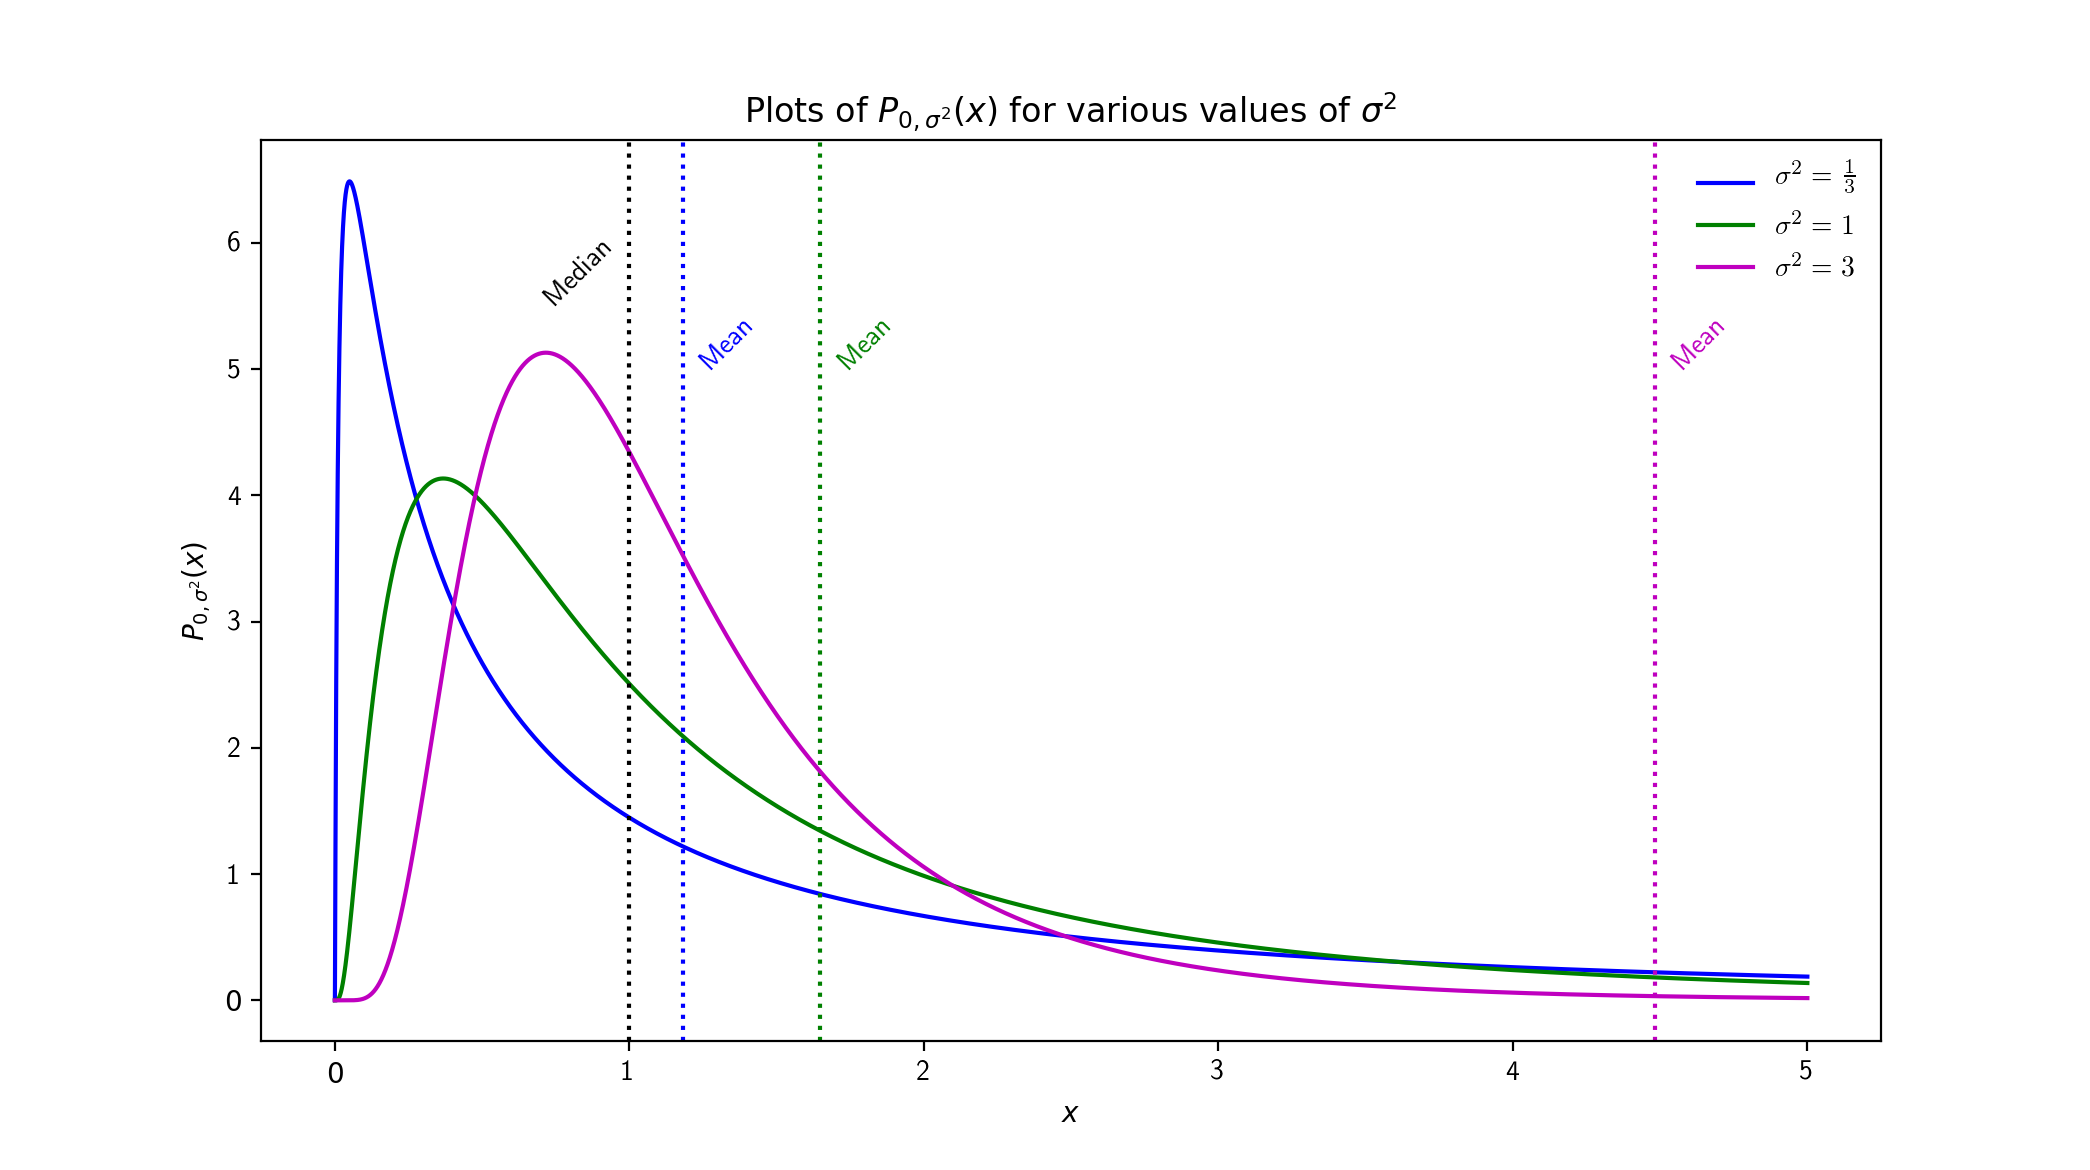
\includegraphics[width=\textwidth]{Problem_10_Plots.png}
            \caption{Plot for 10.4}
            \label{fig:plots_10_4}
        \end{figure}
\end{itemize}
\section*{11. Jensen's Inequality}
Let $ f \colon \R \supset G \to \R $, $ x \mapsto f(x) $ be a function which is convex and differentiable on the connected domain $ G $. As a consequence, for all $ x, x_0 \in G $ we have
\begin{equation}
    f(x) \geq f(x_0) + f'(x_0)(x - x_0).
\end{equation}
\begin{itemize}
    \item[1.] Draw an educationally pristine graph to illustrate that the inequality makes sense as a definition of convexity.
        \begin{problem}
            I am not dedicated enough to draw this with \LaTeX\ and even though my hand-drawn art isn't that great, it's a lot faster.
            \vspace{100mm}
        \end{problem}
    \item[2.] Let $ X $ be a continuous random variable and $ f(x) $ be a convex (differentiable) function. Prove Jensen's inequality:
        \begin{equation}
            \ev{f(X)} \geq f(\ev{X}),
        \end{equation}
        where the average is taken over whatever p-density underlies the randomness of $ X $.
        \begin{problem}
            Let's work with a line tangent to $ f(X) $ at $ \ev{X} = \mu $. This line can be written as
            \begin{equation}
                L(X) = f(\mu) + f'(\mu)(X - \mu) = (f(\mu) - f'(\mu)(\mu)) + f'(\mu)(X) = a + bX
            \end{equation}
            If $ f $ is convex, we know from the above definition that
            \begin{equation}
                \ev{f(X)} \geq \ev{L(X)}
            \end{equation}
            Since the expectation value is a linear functional, we can perform the following operations:
            \begin{equation}
                \ev{f(X)} \geq \ev{L(X)} = \ev{a + bX} = a + b \ev{X} = L(\ev{X}) = f(\ev{X})
            \end{equation}
            The last step works because we defined the line to be tangent to $ f $ at $ \ev{X} $, so it will have the same value there. 
        \end{problem}
\end{itemize}

\end{document}
